\subsubsection{Ausgewählte Untersuchungsgebiete für Referenzszenario (Nr. 1)}\label{chap_scenario_1_ausgewählte_untersuchungsgebiete}
Alle Untersuchungsgebiete, in denen Zügen der folgenden Kategorie(n) verkehren (siehe auch Abbildung \ref{fig_s_1_ausgewählte_untersuchungsgebiete}):
\begin{itemize}
    \item \acrlong{sgv}
\end{itemize}

Hinweis: Für Gebiete mit \acrshort{sgv} werden die Traktionsfälle Batterie und Wasserstoff nicht gerechnet.

\begin{center}
	\begin{figure}[p]
	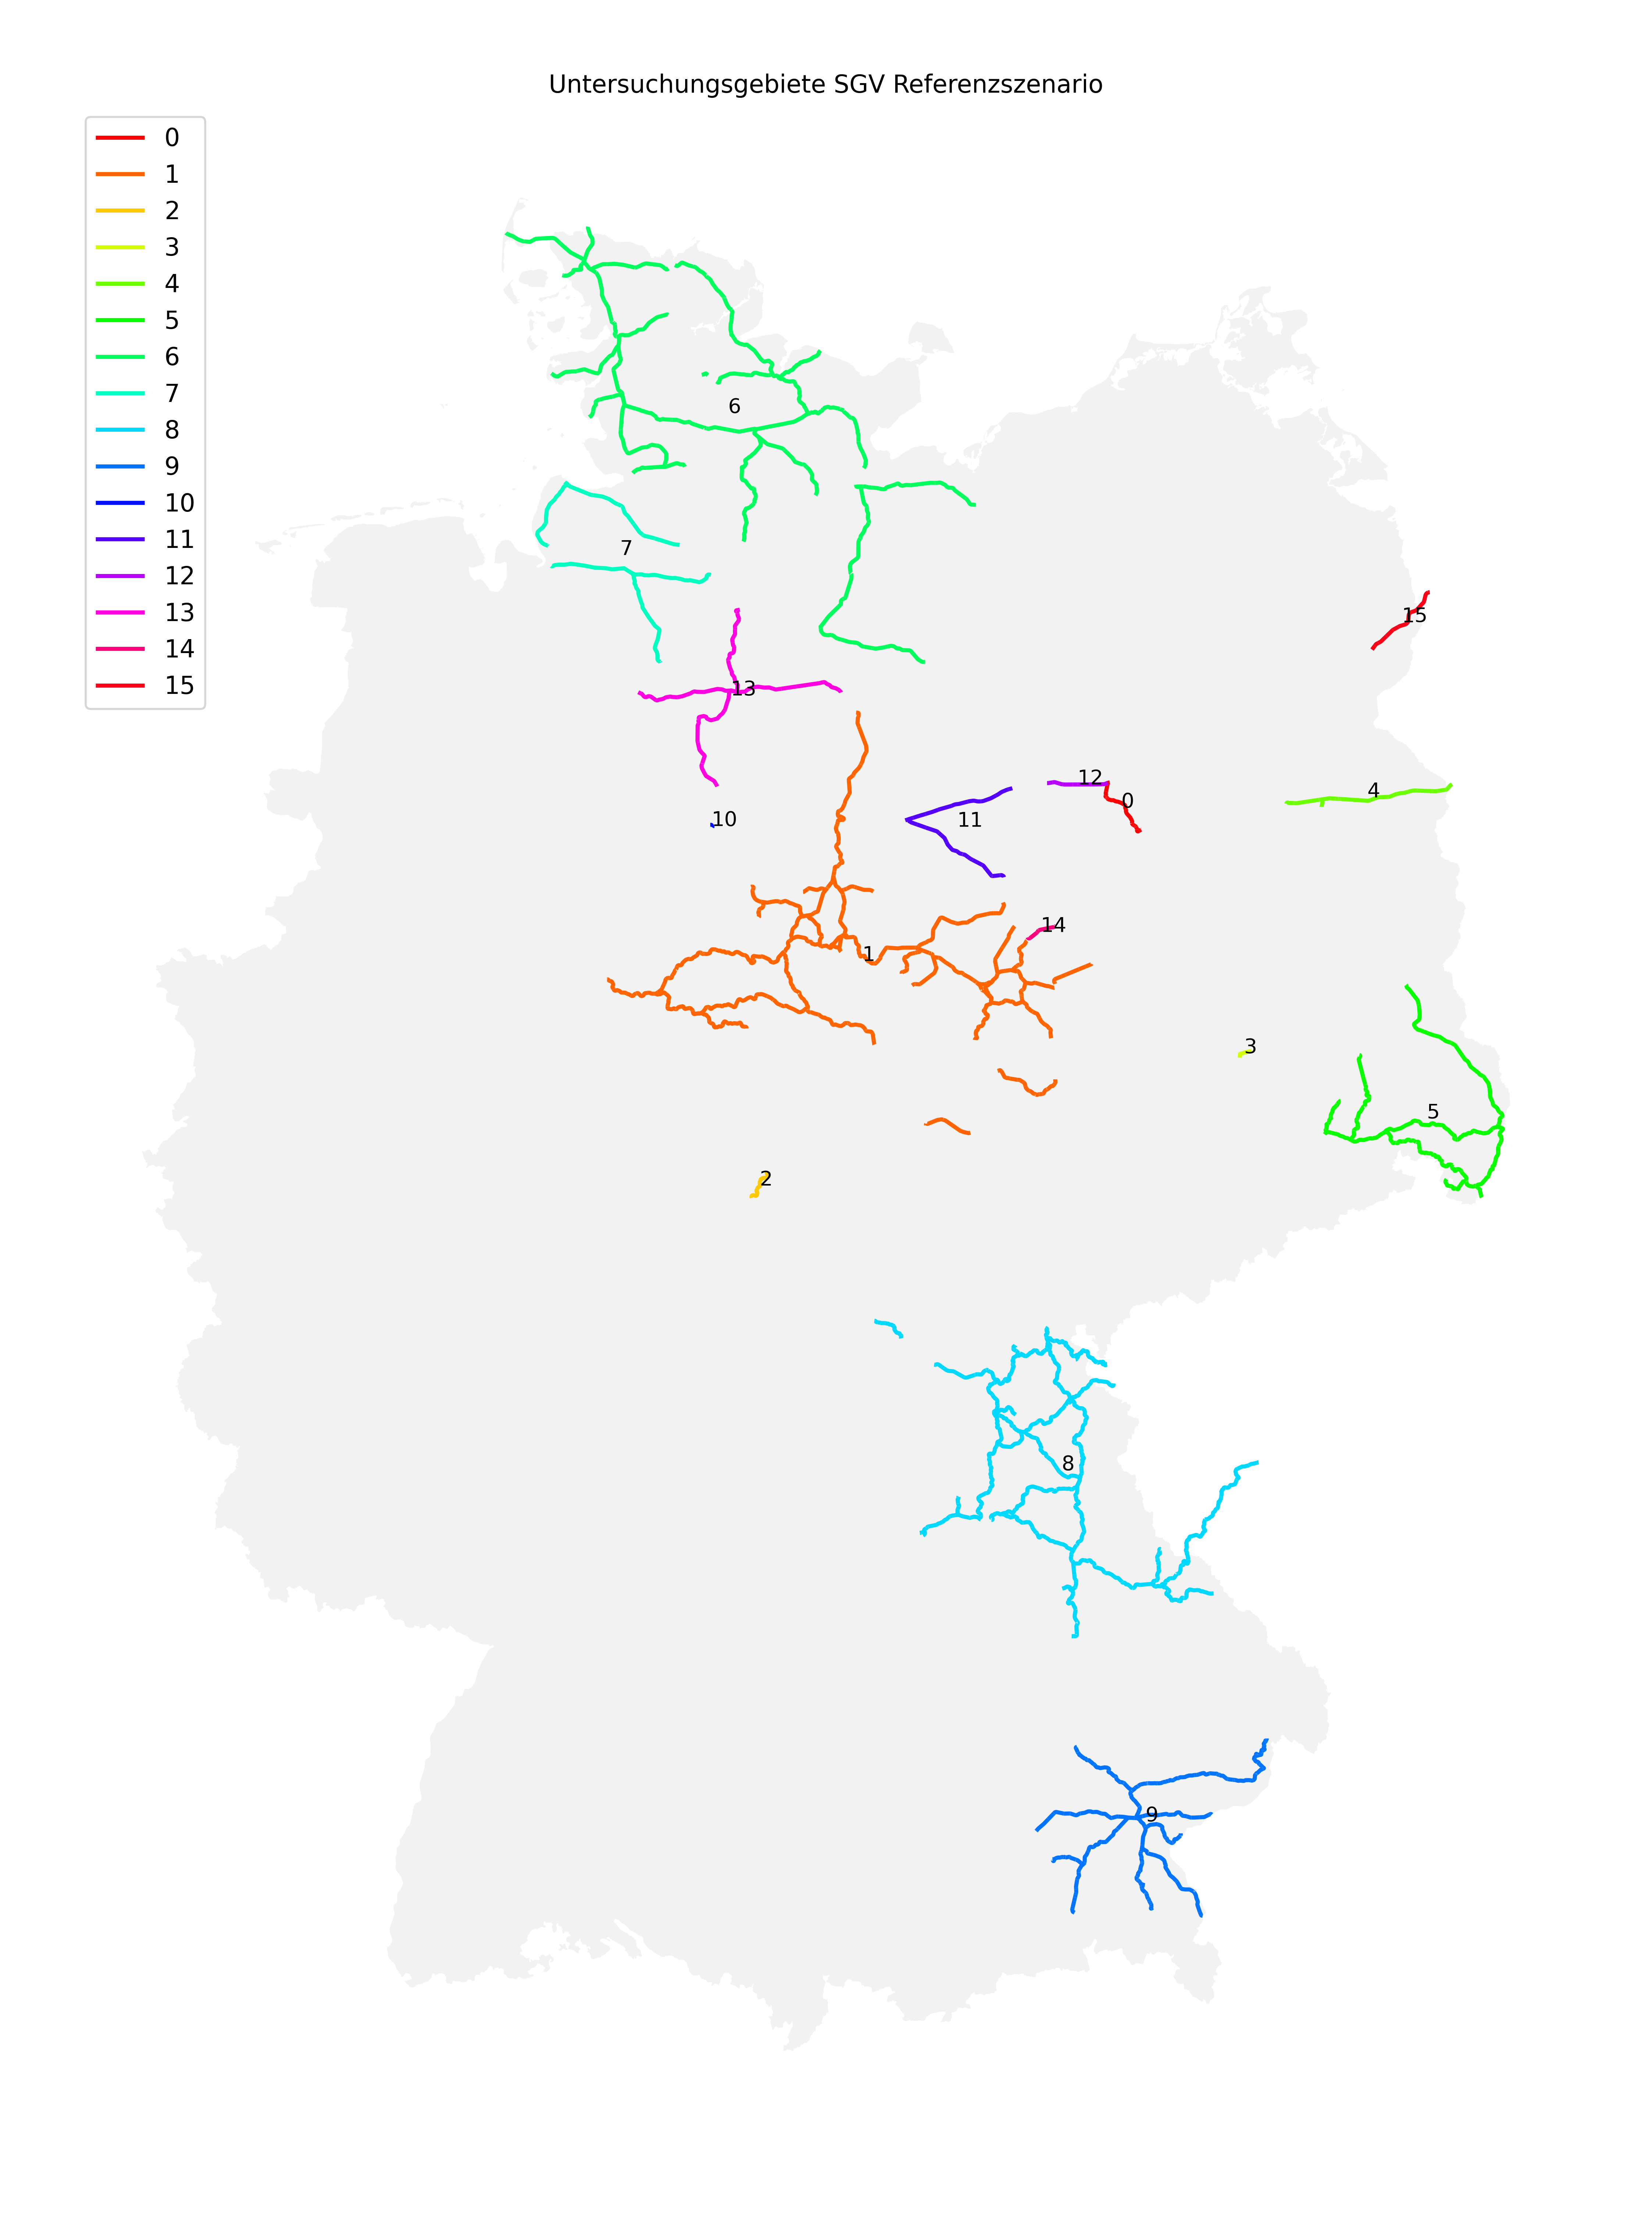
\includegraphics[height=0.85\textheight]{../report_scenarios/s_1/files/master_areas_sgv}
	\caption{\label{fig_s_1_ausgewählte_untersuchungsgebiete} Ausgewählte Untersuchungsgebiete für Szenario 1}
	\end{figure}
\end{center}


\begin{center}
\captionof{table}{\label{table_1_übersicht_untersuchungsgebiet_1} Übersicht ausgewählte Untersuchungsgebiete Szenrio 1}
\begin{tabularx}{\textwidth}{l | X | X | X | X} Nummer & kosteneffizienteste Traktion & Gesamtkosten kosteneffizienteste Traktion & Gesamtkosten e-Fuel & Gesamtkosten Diesel \\
\hline
0 &optimised electrification &
\SI{102121}{Tsd. \EUR} &
\SI{290288}{Tsd. \EUR} &
\SI{263339}{Tsd. \EUR} \\
1 &optimised electrification &
\SI{2214842}{Tsd. \EUR} &
\SI{4067278}{Tsd. \EUR} &
\SI{3999033}{Tsd. \EUR} \\
2 &electrification &
\SI{102705}{Tsd. \EUR} &
\SI{274835}{Tsd. \EUR} &
\SI{238453}{Tsd. \EUR} \\
3 &electrification &
\SI{43307}{Tsd. \EUR} &
\SI{112878}{Tsd. \EUR} &
\SI{98550}{Tsd. \EUR} \\
4 &electrification &
\SI{290937}{Tsd. \EUR} &
\SI{569624}{Tsd. \EUR} &
\SI{556122}{Tsd. \EUR} \\
5 &optimised electrification &
\SI{1014305}{Tsd. \EUR} &
\SI{1870642}{Tsd. \EUR} &
\SI{1936918}{Tsd. \EUR} \\
6 &optimised electrification &
\SI{3944682}{Tsd. \EUR} &
\SI{10724074}{Tsd. \EUR} &
\SI{10178866}{Tsd. \EUR} \\
7 &optimised electrification &
\SI{825159}{Tsd. \EUR} &
\SI{2127587}{Tsd. \EUR} &
\SI{2015965}{Tsd. \EUR} \\
8 &optimised electrification &
\SI{4230667}{Tsd. \EUR} &
\SI{9477572}{Tsd. \EUR} &
\SI{9050737}{Tsd. \EUR} \\
9 &optimised electrification &
\SI{2558631}{Tsd. \EUR} &
\SI{7467403}{Tsd. \EUR} &
\SI{7046026}{Tsd. \EUR} \\
10 &electrification &
\SI{11604}{Tsd. \EUR} &
\SI{27962}{Tsd. \EUR} &
\SI{24848}{Tsd. \EUR} \\
11 &electrification &
\SI{589104}{Tsd. \EUR} &
\SI{1802905}{Tsd. \EUR} &
\SI{1793453}{Tsd. \EUR} \\
12 &electrification &
\SI{314459}{Tsd. \EUR} &
\SI{918875}{Tsd. \EUR} &
\SI{898321}{Tsd. \EUR} \\
13 &optimised electrification &
\SI{734456}{Tsd. \EUR} &
\SI{1860553}{Tsd. \EUR} &
\SI{1708442}{Tsd. \EUR} \\
14 &electrification &
\SI{585361}{Tsd. \EUR} &
\SI{2248625}{Tsd. \EUR} &
\SI{2293446}{Tsd. \EUR} \\
15 &electrification &
\SI{468839}{Tsd. \EUR} &
\SI{1410691}{Tsd. \EUR} &
\SI{1384173}{Tsd. \EUR} \\
\end{tabularx}
\end{center}



	\paragraph*{Untersuchungsgebiet 0}\mbox{} \\
	\captionof{table}{\label{table_1_kenngrößen_untersuchungsgebiet_17278} Basiskenngrößen Untersuchungsgebiet 0}
	\begin{center}
		\begin{tabularx}{\textwidth}{X | r } Kenngröße & Wert \\
		\hline
		Länge & \SI{33.954}{\km} \\
		gewählte Traktion & optimised electrification \\
		Infrastrukturkosten gewählte Traktion (Barwert) & \SI{5559}{Tsd. \EUR} \\
		Betriebskosten gewählte Traktion (Barwert) & \SI{96563}{Tsd. \EUR}\\
		Gesamtkosten gewählte Traktion (Barwert) & \SI{102121}{Tsd. \EUR} \\
		\ce{CO2}-Jahresbilanz Ausgangssituation & \SI{9723}{\tonne} \ce{CO2} \\
		\ce{CO2}-Jahresbilanz Szenario & \SI{272}{\tonne} \ce{CO2} \\
		\end{tabularx}
	\end{center}

	\captionof{table}{\label{table_1_kosten_untersuchungsgebiet_17278} Kosten Untersuchungsgebiet verschiedene Traktionen 0}
	\begin{center}
		\begin{tabularx}{\textwidth}{X | X | X | X} Traktion & Infrastrukturkosten & Betriebskosten & Gesamtkosten\\
		\hline
									electrification & \SI{32994}{Tsd. \EUR} & \SI{87261}{Tsd. \EUR} & \SI{120255}{Tsd. \EUR}\\
												efuel & \SI{1556}{Tsd. \EUR} & \SI{288732}{Tsd. \EUR} & \SI{290288}{Tsd. \EUR}\\
																	optimised electrification & \SI{5559}{Tsd. \EUR} & \SI{96563}{Tsd. \EUR} & \SI{102121}{Tsd. \EUR}\\
												diesel & \SI{1556}{Tsd. \EUR} & \SI{261783}{Tsd. \EUR} & \SI{263339}{Tsd. \EUR}\\
												\end{tabularx}
	\end{center}
	\bigskip

	
\textit{Untersuchungsgebiet ID in Datenbank 17278}
	\paragraph*{Untersuchungsgebiet 1}\mbox{} \\
	\captionof{table}{\label{table_1_kenngrößen_untersuchungsgebiet_17096} Basiskenngrößen Untersuchungsgebiet 1}
	\begin{center}
		\begin{tabularx}{\textwidth}{X | r } Kenngröße & Wert \\
		\hline
		Länge & \SI{1049.579}{\km} \\
		gewählte Traktion & optimised electrification \\
		Infrastrukturkosten gewählte Traktion (Barwert) & \SI{589234}{Tsd. \EUR} \\
		Betriebskosten gewählte Traktion (Barwert) & \SI{1625608}{Tsd. \EUR}\\
		Gesamtkosten gewählte Traktion (Barwert) & \SI{2214842}{Tsd. \EUR} \\
		\ce{CO2}-Jahresbilanz Ausgangssituation & \SI{139646}{\tonne} \ce{CO2} \\
		\ce{CO2}-Jahresbilanz Szenario & \SI{3330}{\tonne} \ce{CO2} \\
		\end{tabularx}
	\end{center}

	\captionof{table}{\label{table_1_kosten_untersuchungsgebiet_17096} Kosten Untersuchungsgebiet verschiedene Traktionen 1}
	\begin{center}
		\begin{tabularx}{\textwidth}{X | X | X | X} Traktion & Infrastrukturkosten & Betriebskosten & Gesamtkosten\\
		\hline
									electrification & \SI{1334201}{Tsd. \EUR} & \SI{1368983}{Tsd. \EUR} & \SI{2703183}{Tsd. \EUR}\\
												efuel & \SI{42021}{Tsd. \EUR} & \SI{4025257}{Tsd. \EUR} & \SI{4067278}{Tsd. \EUR}\\
																	optimised electrification & \SI{589234}{Tsd. \EUR} & \SI{1625608}{Tsd. \EUR} & \SI{2214842}{Tsd. \EUR}\\
												diesel & \SI{42021}{Tsd. \EUR} & \SI{3957012}{Tsd. \EUR} & \SI{3999033}{Tsd. \EUR}\\
												\end{tabularx}
	\end{center}
	\bigskip

	
\textit{Untersuchungsgebiet ID in Datenbank 17096}
	\paragraph*{Untersuchungsgebiet 2}\mbox{} \\
	\captionof{table}{\label{table_1_kenngrößen_untersuchungsgebiet_17281} Basiskenngrößen Untersuchungsgebiet 2}
	\begin{center}
		\begin{tabularx}{\textwidth}{X | r } Kenngröße & Wert \\
		\hline
		Länge & \SI{17.785}{\km} \\
		gewählte Traktion & electrification \\
		Infrastrukturkosten gewählte Traktion (Barwert) & \SI{17282}{Tsd. \EUR} \\
		Betriebskosten gewählte Traktion (Barwert) & \SI{85423}{Tsd. \EUR}\\
		Gesamtkosten gewählte Traktion (Barwert) & \SI{102705}{Tsd. \EUR} \\
		\ce{CO2}-Jahresbilanz Ausgangssituation & \SI{8508}{\tonne} \ce{CO2} \\
		\ce{CO2}-Jahresbilanz Szenario & \SI{252}{\tonne} \ce{CO2} \\
		\end{tabularx}
	\end{center}

	\captionof{table}{\label{table_1_kosten_untersuchungsgebiet_17281} Kosten Untersuchungsgebiet verschiedene Traktionen 2}
	\begin{center}
		\begin{tabularx}{\textwidth}{X | X | X | X} Traktion & Infrastrukturkosten & Betriebskosten & Gesamtkosten\\
		\hline
									electrification & \SI{17282}{Tsd. \EUR} & \SI{85423}{Tsd. \EUR} & \SI{102705}{Tsd. \EUR}\\
												efuel & \SI{1556}{Tsd. \EUR} & \SI{273279}{Tsd. \EUR} & \SI{274835}{Tsd. \EUR}\\
																	optimised electrification & \SI{18790}{Tsd. \EUR} & \SI{85423}{Tsd. \EUR} & \SI{104213}{Tsd. \EUR}\\
												diesel & \SI{1556}{Tsd. \EUR} & \SI{236897}{Tsd. \EUR} & \SI{238453}{Tsd. \EUR}\\
												\end{tabularx}
	\end{center}
	\bigskip

	
\textit{Untersuchungsgebiet ID in Datenbank 17281}
	\paragraph*{Untersuchungsgebiet 3}\mbox{} \\
	\captionof{table}{\label{table_1_kenngrößen_untersuchungsgebiet_17542} Basiskenngrößen Untersuchungsgebiet 3}
	\begin{center}
		\begin{tabularx}{\textwidth}{X | r } Kenngröße & Wert \\
		\hline
		Länge & \SI{6.779}{\km} \\
		gewählte Traktion & electrification \\
		Infrastrukturkosten gewählte Traktion (Barwert) & \SI{6587}{Tsd. \EUR} \\
		Betriebskosten gewählte Traktion (Barwert) & \SI{36720}{Tsd. \EUR}\\
		Gesamtkosten gewählte Traktion (Barwert) & \SI{43307}{Tsd. \EUR} \\
		\ce{CO2}-Jahresbilanz Ausgangssituation & \SI{3352}{\tonne} \ce{CO2} \\
		\ce{CO2}-Jahresbilanz Szenario & \SI{100}{\tonne} \ce{CO2} \\
		\end{tabularx}
	\end{center}

	\captionof{table}{\label{table_1_kosten_untersuchungsgebiet_17542} Kosten Untersuchungsgebiet verschiedene Traktionen 3}
	\begin{center}
		\begin{tabularx}{\textwidth}{X | X | X | X} Traktion & Infrastrukturkosten & Betriebskosten & Gesamtkosten\\
		\hline
									electrification & \SI{6587}{Tsd. \EUR} & \SI{36720}{Tsd. \EUR} & \SI{43307}{Tsd. \EUR}\\
												efuel & \SI{1556}{Tsd. \EUR} & \SI{111322}{Tsd. \EUR} & \SI{112878}{Tsd. \EUR}\\
																	optimised electrification & \SI{8095}{Tsd. \EUR} & \SI{36720}{Tsd. \EUR} & \SI{44815}{Tsd. \EUR}\\
												diesel & \SI{1556}{Tsd. \EUR} & \SI{96994}{Tsd. \EUR} & \SI{98550}{Tsd. \EUR}\\
												\end{tabularx}
	\end{center}
	\bigskip

	
\textit{Untersuchungsgebiet ID in Datenbank 17542}
	\paragraph*{Untersuchungsgebiet 4}\mbox{} \\
	\captionof{table}{\label{table_1_kenngrößen_untersuchungsgebiet_17421} Basiskenngrößen Untersuchungsgebiet 4}
	\begin{center}
		\begin{tabularx}{\textwidth}{X | r } Kenngröße & Wert \\
		\hline
		Länge & \SI{82.795}{\km} \\
		gewählte Traktion & electrification \\
		Infrastrukturkosten gewählte Traktion (Barwert) & \SI{95729}{Tsd. \EUR} \\
		Betriebskosten gewählte Traktion (Barwert) & \SI{195207}{Tsd. \EUR}\\
		Gesamtkosten gewählte Traktion (Barwert) & \SI{290937}{Tsd. \EUR} \\
		\ce{CO2}-Jahresbilanz Ausgangssituation & \SI{19447}{\tonne} \ce{CO2} \\
		\ce{CO2}-Jahresbilanz Szenario & \SI{451}{\tonne} \ce{CO2} \\
		\end{tabularx}
	\end{center}

	\captionof{table}{\label{table_1_kosten_untersuchungsgebiet_17421} Kosten Untersuchungsgebiet verschiedene Traktionen 4}
	\begin{center}
		\begin{tabularx}{\textwidth}{X | X | X | X} Traktion & Infrastrukturkosten & Betriebskosten & Gesamtkosten\\
		\hline
									electrification & \SI{95729}{Tsd. \EUR} & \SI{195207}{Tsd. \EUR} & \SI{290937}{Tsd. \EUR}\\
												efuel & \SI{4669}{Tsd. \EUR} & \SI{564955}{Tsd. \EUR} & \SI{569624}{Tsd. \EUR}\\
																	optimised electrification & \SI{98744}{Tsd. \EUR} & \SI{195207}{Tsd. \EUR} & \SI{293952}{Tsd. \EUR}\\
												diesel & \SI{4669}{Tsd. \EUR} & \SI{551453}{Tsd. \EUR} & \SI{556122}{Tsd. \EUR}\\
												\end{tabularx}
	\end{center}
	\bigskip

	
\textit{Untersuchungsgebiet ID in Datenbank 17421}
	\paragraph*{Untersuchungsgebiet 5}\mbox{} \\
	\captionof{table}{\label{table_1_kenngrößen_untersuchungsgebiet_17443} Basiskenngrößen Untersuchungsgebiet 5}
	\begin{center}
		\begin{tabularx}{\textwidth}{X | r } Kenngröße & Wert \\
		\hline
		Länge & \SI{373.393}{\km} \\
		gewählte Traktion & optimised electrification \\
		Infrastrukturkosten gewählte Traktion (Barwert) & \SI{150078}{Tsd. \EUR} \\
		Betriebskosten gewählte Traktion (Barwert) & \SI{864227}{Tsd. \EUR}\\
		Gesamtkosten gewählte Traktion (Barwert) & \SI{1014305}{Tsd. \EUR} \\
		\ce{CO2}-Jahresbilanz Ausgangssituation & \SI{67404}{\tonne} \ce{CO2} \\
		\ce{CO2}-Jahresbilanz Szenario & \SI{1532}{\tonne} \ce{CO2} \\
		\end{tabularx}
	\end{center}

	\captionof{table}{\label{table_1_kosten_untersuchungsgebiet_17443} Kosten Untersuchungsgebiet verschiedene Traktionen 5}
	\begin{center}
		\begin{tabularx}{\textwidth}{X | X | X | X} Traktion & Infrastrukturkosten & Betriebskosten & Gesamtkosten\\
		\hline
									electrification & \SI{466400}{Tsd. \EUR} & \SI{652723}{Tsd. \EUR} & \SI{1119122}{Tsd. \EUR}\\
												efuel & \SI{15563}{Tsd. \EUR} & \SI{1855079}{Tsd. \EUR} & \SI{1870642}{Tsd. \EUR}\\
																	optimised electrification & \SI{150078}{Tsd. \EUR} & \SI{864227}{Tsd. \EUR} & \SI{1014305}{Tsd. \EUR}\\
												diesel & \SI{15563}{Tsd. \EUR} & \SI{1921354}{Tsd. \EUR} & \SI{1936918}{Tsd. \EUR}\\
												\end{tabularx}
	\end{center}
	\bigskip

	
\textit{Untersuchungsgebiet ID in Datenbank 17443}
	\paragraph*{Untersuchungsgebiet 6}\mbox{} \\
	\captionof{table}{\label{table_1_kenngrößen_untersuchungsgebiet_17760} Basiskenngrößen Untersuchungsgebiet 6}
	\begin{center}
		\begin{tabularx}{\textwidth}{X | r } Kenngröße & Wert \\
		\hline
		Länge & \SI{934.462}{\km} \\
		gewählte Traktion & optimised electrification \\
		Infrastrukturkosten gewählte Traktion (Barwert) & \SI{581412}{Tsd. \EUR} \\
		Betriebskosten gewählte Traktion (Barwert) & \SI{3363270}{Tsd. \EUR}\\
		Gesamtkosten gewählte Traktion (Barwert) & \SI{3944682}{Tsd. \EUR} \\
		\ce{CO2}-Jahresbilanz Ausgangssituation & \SI{364434}{\tonne} \ce{CO2} \\
		\ce{CO2}-Jahresbilanz Szenario & \SI{7784}{\tonne} \ce{CO2} \\
		\end{tabularx}
	\end{center}

	\captionof{table}{\label{table_1_kosten_untersuchungsgebiet_17760} Kosten Untersuchungsgebiet verschiedene Traktionen 6}
	\begin{center}
		\begin{tabularx}{\textwidth}{X | X | X | X} Traktion & Infrastrukturkosten & Betriebskosten & Gesamtkosten\\
		\hline
									electrification & \SI{1050753}{Tsd. \EUR} & \SI{3146027}{Tsd. \EUR} & \SI{4196780}{Tsd. \EUR}\\
												efuel & \SI{37352}{Tsd. \EUR} & \SI{10686722}{Tsd. \EUR} & \SI{10724074}{Tsd. \EUR}\\
																	optimised electrification & \SI{581412}{Tsd. \EUR} & \SI{3363270}{Tsd. \EUR} & \SI{3944682}{Tsd. \EUR}\\
												diesel & \SI{37352}{Tsd. \EUR} & \SI{10141514}{Tsd. \EUR} & \SI{10178866}{Tsd. \EUR}\\
												\end{tabularx}
	\end{center}
	\bigskip

	
\textit{Untersuchungsgebiet ID in Datenbank 17760}
	\paragraph*{Untersuchungsgebiet 7}\mbox{} \\
	\captionof{table}{\label{table_1_kenngrößen_untersuchungsgebiet_17226} Basiskenngrößen Untersuchungsgebiet 7}
	\begin{center}
		\begin{tabularx}{\textwidth}{X | r } Kenngröße & Wert \\
		\hline
		Länge & \SI{219.697}{\km} \\
		gewählte Traktion & optimised electrification \\
		Infrastrukturkosten gewählte Traktion (Barwert) & \SI{199911}{Tsd. \EUR} \\
		Betriebskosten gewählte Traktion (Barwert) & \SI{625248}{Tsd. \EUR}\\
		Gesamtkosten gewählte Traktion (Barwert) & \SI{825159}{Tsd. \EUR} \\
		\ce{CO2}-Jahresbilanz Ausgangssituation & \SI{75426}{\tonne} \ce{CO2} \\
		\ce{CO2}-Jahresbilanz Szenario & \SI{1726}{\tonne} \ce{CO2} \\
		\end{tabularx}
	\end{center}

	\captionof{table}{\label{table_1_kosten_untersuchungsgebiet_17226} Kosten Untersuchungsgebiet verschiedene Traktionen 7}
	\begin{center}
		\begin{tabularx}{\textwidth}{X | X | X | X} Traktion & Infrastrukturkosten & Betriebskosten & Gesamtkosten\\
		\hline
									electrification & \SI{267876}{Tsd. \EUR} & \SI{592392}{Tsd. \EUR} & \SI{860268}{Tsd. \EUR}\\
												efuel & \SI{9338}{Tsd. \EUR} & \SI{2118249}{Tsd. \EUR} & \SI{2127587}{Tsd. \EUR}\\
																	optimised electrification & \SI{199911}{Tsd. \EUR} & \SI{625248}{Tsd. \EUR} & \SI{825159}{Tsd. \EUR}\\
												diesel & \SI{9338}{Tsd. \EUR} & \SI{2006627}{Tsd. \EUR} & \SI{2015965}{Tsd. \EUR}\\
												\end{tabularx}
	\end{center}
	\bigskip

	
\textit{Untersuchungsgebiet ID in Datenbank 17226}
	\paragraph*{Untersuchungsgebiet 8}\mbox{} \\
	\captionof{table}{\label{table_1_kenngrößen_untersuchungsgebiet_17656} Basiskenngrößen Untersuchungsgebiet 8}
	\begin{center}
		\begin{tabularx}{\textwidth}{X | r } Kenngröße & Wert \\
		\hline
		Länge & \SI{929.157}{\km} \\
		gewählte Traktion & optimised electrification \\
		Infrastrukturkosten gewählte Traktion (Barwert) & \SI{1208939}{Tsd. \EUR} \\
		Betriebskosten gewählte Traktion (Barwert) & \SI{3021728}{Tsd. \EUR}\\
		Gesamtkosten gewählte Traktion (Barwert) & \SI{4230667}{Tsd. \EUR} \\
		\ce{CO2}-Jahresbilanz Ausgangssituation & \SI{330550}{\tonne} \ce{CO2} \\
		\ce{CO2}-Jahresbilanz Szenario & \SI{7632}{\tonne} \ce{CO2} \\
		\end{tabularx}
	\end{center}

	\captionof{table}{\label{table_1_kosten_untersuchungsgebiet_17656} Kosten Untersuchungsgebiet verschiedene Traktionen 8}
	\begin{center}
		\begin{tabularx}{\textwidth}{X | X | X | X} Traktion & Infrastrukturkosten & Betriebskosten & Gesamtkosten\\
		\hline
									electrification & \SI{1348298}{Tsd. \EUR} & \SI{2946000}{Tsd. \EUR} & \SI{4294299}{Tsd. \EUR}\\
												efuel & \SI{37352}{Tsd. \EUR} & \SI{9440220}{Tsd. \EUR} & \SI{9477572}{Tsd. \EUR}\\
																	optimised electrification & \SI{1208939}{Tsd. \EUR} & \SI{3021728}{Tsd. \EUR} & \SI{4230667}{Tsd. \EUR}\\
												diesel & \SI{37352}{Tsd. \EUR} & \SI{9013386}{Tsd. \EUR} & \SI{9050737}{Tsd. \EUR}\\
												\end{tabularx}
	\end{center}
	\bigskip

	
\textit{Untersuchungsgebiet ID in Datenbank 17656}
	\paragraph*{Untersuchungsgebiet 9}\mbox{} \\
	\captionof{table}{\label{table_1_kenngrößen_untersuchungsgebiet_17308} Basiskenngrößen Untersuchungsgebiet 9}
	\begin{center}
		\begin{tabularx}{\textwidth}{X | r } Kenngröße & Wert \\
		\hline
		Länge & \SI{450.258}{\km} \\
		gewählte Traktion & optimised electrification \\
		Infrastrukturkosten gewählte Traktion (Barwert) & \SI{286976}{Tsd. \EUR} \\
		Betriebskosten gewählte Traktion (Barwert) & \SI{2271655}{Tsd. \EUR}\\
		Gesamtkosten gewählte Traktion (Barwert) & \SI{2558631}{Tsd. \EUR} \\
		\ce{CO2}-Jahresbilanz Ausgangssituation & \SI{254590}{\tonne} \ce{CO2} \\
		\ce{CO2}-Jahresbilanz Szenario & \SI{5578}{\tonne} \ce{CO2} \\
		\end{tabularx}
	\end{center}

	\captionof{table}{\label{table_1_kosten_untersuchungsgebiet_17308} Kosten Untersuchungsgebiet verschiedene Traktionen 9}
	\begin{center}
		\begin{tabularx}{\textwidth}{X | X | X | X} Traktion & Infrastrukturkosten & Betriebskosten & Gesamtkosten\\
		\hline
									electrification & \SI{454110}{Tsd. \EUR} & \SI{2198890}{Tsd. \EUR} & \SI{2653001}{Tsd. \EUR}\\
												efuel & \SI{18676}{Tsd. \EUR} & \SI{7448727}{Tsd. \EUR} & \SI{7467403}{Tsd. \EUR}\\
																	optimised electrification & \SI{286976}{Tsd. \EUR} & \SI{2271655}{Tsd. \EUR} & \SI{2558631}{Tsd. \EUR}\\
												diesel & \SI{18676}{Tsd. \EUR} & \SI{7027350}{Tsd. \EUR} & \SI{7046026}{Tsd. \EUR}\\
												\end{tabularx}
	\end{center}
	\bigskip

	
\textit{Untersuchungsgebiet ID in Datenbank 17308}
	\paragraph*{Untersuchungsgebiet 10}\mbox{} \\
	\captionof{table}{\label{table_1_kenngrößen_untersuchungsgebiet_17283} Basiskenngrößen Untersuchungsgebiet 10}
	\begin{center}
		\begin{tabularx}{\textwidth}{X | r } Kenngröße & Wert \\
		\hline
		Länge & \SI{1.79}{\km} \\
		gewählte Traktion & electrification \\
		Infrastrukturkosten gewählte Traktion (Barwert) & \SI{1739}{Tsd. \EUR} \\
		Betriebskosten gewählte Traktion (Barwert) & \SI{9864}{Tsd. \EUR}\\
		Gesamtkosten gewählte Traktion (Barwert) & \SI{11604}{Tsd. \EUR} \\
		\ce{CO2}-Jahresbilanz Ausgangssituation & \SI{726}{\tonne} \ce{CO2} \\
		\ce{CO2}-Jahresbilanz Szenario & \SI{22}{\tonne} \ce{CO2} \\
		\end{tabularx}
	\end{center}

	\captionof{table}{\label{table_1_kosten_untersuchungsgebiet_17283} Kosten Untersuchungsgebiet verschiedene Traktionen 10}
	\begin{center}
		\begin{tabularx}{\textwidth}{X | X | X | X} Traktion & Infrastrukturkosten & Betriebskosten & Gesamtkosten\\
		\hline
									electrification & \SI{1739}{Tsd. \EUR} & \SI{9864}{Tsd. \EUR} & \SI{11604}{Tsd. \EUR}\\
												efuel & \SI{1556}{Tsd. \EUR} & \SI{26405}{Tsd. \EUR} & \SI{27962}{Tsd. \EUR}\\
																	optimised electrification & \SI{3247}{Tsd. \EUR} & \SI{9864}{Tsd. \EUR} & \SI{13111}{Tsd. \EUR}\\
												diesel & \SI{1556}{Tsd. \EUR} & \SI{23292}{Tsd. \EUR} & \SI{24848}{Tsd. \EUR}\\
												\end{tabularx}
	\end{center}
	\bigskip

	
\textit{Untersuchungsgebiet ID in Datenbank 17283}
	\paragraph*{Untersuchungsgebiet 11}\mbox{} \\
	\captionof{table}{\label{table_1_kenngrößen_untersuchungsgebiet_17253} Basiskenngrößen Untersuchungsgebiet 11}
	\begin{center}
		\begin{tabularx}{\textwidth}{X | r } Kenngröße & Wert \\
		\hline
		Länge & \SI{106.006}{\km} \\
		gewählte Traktion & electrification \\
		Infrastrukturkosten gewählte Traktion (Barwert) & \SI{103008}{Tsd. \EUR} \\
		Betriebskosten gewählte Traktion (Barwert) & \SI{486096}{Tsd. \EUR}\\
		Gesamtkosten gewählte Traktion (Barwert) & \SI{589104}{Tsd. \EUR} \\
		\ce{CO2}-Jahresbilanz Ausgangssituation & \SI{69075}{\tonne} \ce{CO2} \\
		\ce{CO2}-Jahresbilanz Szenario & \SI{1413}{\tonne} \ce{CO2} \\
		\end{tabularx}
	\end{center}

	\captionof{table}{\label{table_1_kosten_untersuchungsgebiet_17253} Kosten Untersuchungsgebiet verschiedene Traktionen 11}
	\begin{center}
		\begin{tabularx}{\textwidth}{X | X | X | X} Traktion & Infrastrukturkosten & Betriebskosten & Gesamtkosten\\
		\hline
									electrification & \SI{103008}{Tsd. \EUR} & \SI{486096}{Tsd. \EUR} & \SI{589104}{Tsd. \EUR}\\
												efuel & \SI{4669}{Tsd. \EUR} & \SI{1798236}{Tsd. \EUR} & \SI{1802905}{Tsd. \EUR}\\
																	optimised electrification & \SI{104516}{Tsd. \EUR} & \SI{486096}{Tsd. \EUR} & \SI{590612}{Tsd. \EUR}\\
												diesel & \SI{4669}{Tsd. \EUR} & \SI{1788784}{Tsd. \EUR} & \SI{1793453}{Tsd. \EUR}\\
												\end{tabularx}
	\end{center}
	\bigskip

	
\textit{Untersuchungsgebiet ID in Datenbank 17253}
	\paragraph*{Untersuchungsgebiet 12}\mbox{} \\
	\captionof{table}{\label{table_1_kenngrößen_untersuchungsgebiet_17713} Basiskenngrößen Untersuchungsgebiet 12}
	\begin{center}
		\begin{tabularx}{\textwidth}{X | r } Kenngröße & Wert \\
		\hline
		Länge & \SI{27.807}{\km} \\
		gewählte Traktion & electrification \\
		Infrastrukturkosten gewählte Traktion (Barwert) & \SI{27021}{Tsd. \EUR} \\
		Betriebskosten gewählte Traktion (Barwert) & \SI{287438}{Tsd. \EUR}\\
		Gesamtkosten gewählte Traktion (Barwert) & \SI{314459}{Tsd. \EUR} \\
		\ce{CO2}-Jahresbilanz Ausgangssituation & \SI{33260}{\tonne} \ce{CO2} \\
		\ce{CO2}-Jahresbilanz Szenario & \SI{758}{\tonne} \ce{CO2} \\
		\end{tabularx}
	\end{center}

	\captionof{table}{\label{table_1_kosten_untersuchungsgebiet_17713} Kosten Untersuchungsgebiet verschiedene Traktionen 12}
	\begin{center}
		\begin{tabularx}{\textwidth}{X | X | X | X} Traktion & Infrastrukturkosten & Betriebskosten & Gesamtkosten\\
		\hline
									electrification & \SI{27021}{Tsd. \EUR} & \SI{287438}{Tsd. \EUR} & \SI{314459}{Tsd. \EUR}\\
												efuel & \SI{1556}{Tsd. \EUR} & \SI{917319}{Tsd. \EUR} & \SI{918875}{Tsd. \EUR}\\
																	optimised electrification & \SI{27021}{Tsd. \EUR} & \SI{287438}{Tsd. \EUR} & \SI{314459}{Tsd. \EUR}\\
												diesel & \SI{1556}{Tsd. \EUR} & \SI{896765}{Tsd. \EUR} & \SI{898321}{Tsd. \EUR}\\
												\end{tabularx}
	\end{center}
	\bigskip

	
\textit{Untersuchungsgebiet ID in Datenbank 17713}
	\paragraph*{Untersuchungsgebiet 13}\mbox{} \\
	\captionof{table}{\label{table_1_kenngrößen_untersuchungsgebiet_17305} Basiskenngrößen Untersuchungsgebiet 13}
	\begin{center}
		\begin{tabularx}{\textwidth}{X | r } Kenngröße & Wert \\
		\hline
		Länge & \SI{203.153}{\km} \\
		gewählte Traktion & optimised electrification \\
		Infrastrukturkosten gewählte Traktion (Barwert) & \SI{95180}{Tsd. \EUR} \\
		Betriebskosten gewählte Traktion (Barwert) & \SI{639276}{Tsd. \EUR}\\
		Gesamtkosten gewählte Traktion (Barwert) & \SI{734456}{Tsd. \EUR} \\
		\ce{CO2}-Jahresbilanz Ausgangssituation & \SI{63060}{\tonne} \ce{CO2} \\
		\ce{CO2}-Jahresbilanz Szenario & \SI{1706}{\tonne} \ce{CO2} \\
		\end{tabularx}
	\end{center}

	\captionof{table}{\label{table_1_kosten_untersuchungsgebiet_17305} Kosten Untersuchungsgebiet verschiedene Traktionen 13}
	\begin{center}
		\begin{tabularx}{\textwidth}{X | X | X | X} Traktion & Infrastrukturkosten & Betriebskosten & Gesamtkosten\\
		\hline
									electrification & \SI{198721}{Tsd. \EUR} & \SI{567600}{Tsd. \EUR} & \SI{766321}{Tsd. \EUR}\\
												efuel & \SI{9338}{Tsd. \EUR} & \SI{1851215}{Tsd. \EUR} & \SI{1860553}{Tsd. \EUR}\\
																	optimised electrification & \SI{95180}{Tsd. \EUR} & \SI{639276}{Tsd. \EUR} & \SI{734456}{Tsd. \EUR}\\
												diesel & \SI{9338}{Tsd. \EUR} & \SI{1699104}{Tsd. \EUR} & \SI{1708442}{Tsd. \EUR}\\
												\end{tabularx}
	\end{center}
	\bigskip

	
\textit{Untersuchungsgebiet ID in Datenbank 17305}
	\paragraph*{Untersuchungsgebiet 14}\mbox{} \\
	\captionof{table}{\label{table_1_kenngrößen_untersuchungsgebiet_17725} Basiskenngrößen Untersuchungsgebiet 14}
	\begin{center}
		\begin{tabularx}{\textwidth}{X | r } Kenngröße & Wert \\
		\hline
		Länge & \SI{14.43}{\km} \\
		gewählte Traktion & electrification \\
		Infrastrukturkosten gewählte Traktion (Barwert) & \SI{15155}{Tsd. \EUR} \\
		Betriebskosten gewählte Traktion (Barwert) & \SI{570206}{Tsd. \EUR}\\
		Gesamtkosten gewählte Traktion (Barwert) & \SI{585361}{Tsd. \EUR} \\
		\ce{CO2}-Jahresbilanz Ausgangssituation & \SI{86654}{\tonne} \ce{CO2} \\
		\ce{CO2}-Jahresbilanz Szenario & \SI{1432}{\tonne} \ce{CO2} \\
		\end{tabularx}
	\end{center}

	\captionof{table}{\label{table_1_kosten_untersuchungsgebiet_17725} Kosten Untersuchungsgebiet verschiedene Traktionen 14}
	\begin{center}
		\begin{tabularx}{\textwidth}{X | X | X | X} Traktion & Infrastrukturkosten & Betriebskosten & Gesamtkosten\\
		\hline
									electrification & \SI{15155}{Tsd. \EUR} & \SI{570206}{Tsd. \EUR} & \SI{585361}{Tsd. \EUR}\\
												efuel & \SI{1556}{Tsd. \EUR} & \SI{2247069}{Tsd. \EUR} & \SI{2248625}{Tsd. \EUR}\\
																	optimised electrification & \SI{15155}{Tsd. \EUR} & \SI{570206}{Tsd. \EUR} & \SI{585361}{Tsd. \EUR}\\
												diesel & \SI{1556}{Tsd. \EUR} & \SI{2291890}{Tsd. \EUR} & \SI{2293446}{Tsd. \EUR}\\
												\end{tabularx}
	\end{center}
	\bigskip

	
\textit{Untersuchungsgebiet ID in Datenbank 17725}
	\paragraph*{Untersuchungsgebiet 15}\mbox{} \\
	\captionof{table}{\label{table_1_kenngrößen_untersuchungsgebiet_17558} Basiskenngrößen Untersuchungsgebiet 15}
	\begin{center}
		\begin{tabularx}{\textwidth}{X | r } Kenngröße & Wert \\
		\hline
		Länge & \SI{39.444}{\km} \\
		gewählte Traktion & electrification \\
		Infrastrukturkosten gewählte Traktion (Barwert) & \SI{38329}{Tsd. \EUR} \\
		Betriebskosten gewählte Traktion (Barwert) & \SI{430510}{Tsd. \EUR}\\
		Gesamtkosten gewählte Traktion (Barwert) & \SI{468839}{Tsd. \EUR} \\
		\ce{CO2}-Jahresbilanz Ausgangssituation & \SI{49364}{\tonne} \ce{CO2} \\
		\ce{CO2}-Jahresbilanz Szenario & \SI{992}{\tonne} \ce{CO2} \\
		\end{tabularx}
	\end{center}

	\captionof{table}{\label{table_1_kosten_untersuchungsgebiet_17558} Kosten Untersuchungsgebiet verschiedene Traktionen 15}
	\begin{center}
		\begin{tabularx}{\textwidth}{X | X | X | X} Traktion & Infrastrukturkosten & Betriebskosten & Gesamtkosten\\
		\hline
									electrification & \SI{38329}{Tsd. \EUR} & \SI{430510}{Tsd. \EUR} & \SI{468839}{Tsd. \EUR}\\
												efuel & \SI{1556}{Tsd. \EUR} & \SI{1409134}{Tsd. \EUR} & \SI{1410691}{Tsd. \EUR}\\
																	optimised electrification & \SI{39836}{Tsd. \EUR} & \SI{430510}{Tsd. \EUR} & \SI{470346}{Tsd. \EUR}\\
												diesel & \SI{1556}{Tsd. \EUR} & \SI{1382617}{Tsd. \EUR} & \SI{1384173}{Tsd. \EUR}\\
												\end{tabularx}
	\end{center}
	\bigskip

	
\textit{Untersuchungsgebiet ID in Datenbank 17558}
